\chapter{Exercise 12}
The purpose of the exercise is to get an overview of how to setup and work with WebGL. 
WebGL is based on OpenGL ES 2.0, which is a subset of the OpenGL API we have been 
working with so far. We get access to the OpenGL API through a WebGL context object 
that gives us the naming convention we are used to but without the gl-prefix.

\section{Part 1}
Following instructions in the exercise I obtained a program drawing a colored triangle
as in the picture below: \ref{fig:exercise_12_part_3}.
\begin{figure}[ht!]
	\begin{center}
		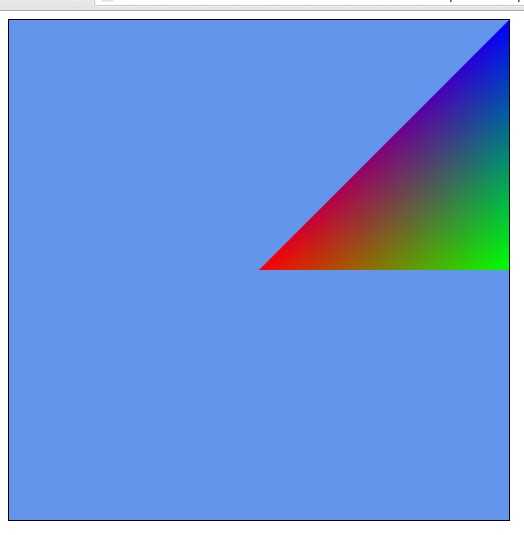
\includegraphics[width=.6\textwidth]{figures/exercise_12_part_3}
	\end{center}
	\vspace{-4.5ex}\caption{Exercise 12 part 3}
	\label{fig:exercise_12_part_3} 
\end{figure}

\section{Part 2}
I managed to implement phong shading per fragment using webgl and the results are below.

\begin{figure}[ht!]
	\begin{center}
		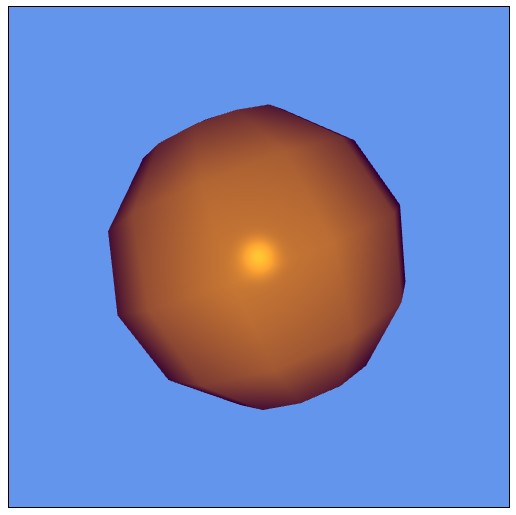
\includegraphics[width=.5\textwidth]{figures/exercise_12_part_4_1}
	\end{center}
	\vspace{-4.5ex}\caption{Exercise 12 part 4 - Point Light}
	\label{fig:exercise_12_part_4_1} 
\end{figure}

\begin{figure}[ht!]
	\begin{center}
		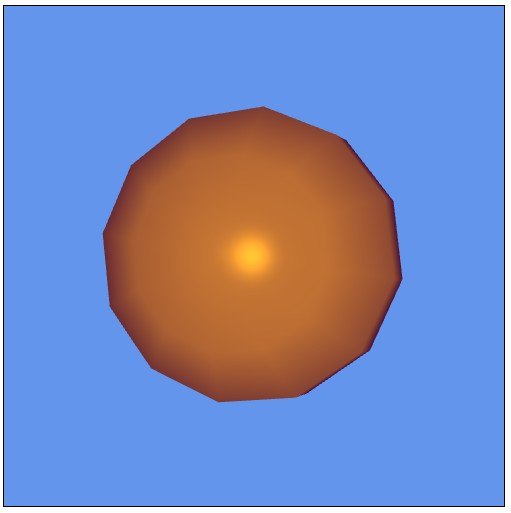
\includegraphics[width=.5\textwidth]{figures/exercise_12_part_4_2}
	\end{center}
	\vspace{-4.5ex}\caption{Exercise 12 part 4 - Directional Light}
	\label{fig:exercise_12_part_4_2} 
\end{figure}
\clearpage
\section{Part 3}
The result of the last part we can see in the picture \ref{fig:exercise_12_part_5}.
\begin{figure}[ht!]
	\begin{center}
		
\includegraphics[width=.6\textwidth]{figures/exercise_12_part_5}
	\end{center}
	\vspace{-4.5ex}\caption{Exercise 12 part 5}
	\label{fig:exercise_12_part_5} 
\end{figure}